\documentclass[a4paper]{article}
\usepackage[margin = 1 in]{geometry}
\usepackage{fancyhdr}
\usepackage{lastpage}
\usepackage{ctex}
\usepackage[utf8]{inputenc} % Required for inputting international characters
\usepackage[T1]{fontenc} % Output font encoding for international characters
\usepackage[sfdefault]{ClearSans} % Use the Clear Sans font (sans serif)
\usepackage{tocloft} 
\usepackage[hidelinks]{hyperref}
\usepackage{makecell}%导入表格宏包
\usepackage{bmpsize}
\usepackage{graphicx}
\usepackage{epstopdf}
\usepackage{caption}
\usepackage{enumitem}
\usepackage{float}
\usepackage{multirow}
\usepackage{makecell}
\usepackage{amsmath} 

\author{Vergil/Zijun Li李子骏}
\title{Week 1}
\date{2023.4.1}

\begin{document}
\maketitle
\noindent基于电商平台数据(user\_data和user\_type)分析平台用户表现现状,同时分析时间维度上是否存在购买量突增和突降情况,并进行归因分析,具体问题如下:

\noindent1. 基础信息: 日PV有多少(浏览人次), 日UV有多少(浏览去重人数),付费率情况如何(付费人数/浏览人数), 复购率是多少(购买2次以上人数/购买人数),漏斗流失情况如何(浏览、收藏、加购物车、购买每一步漏斗的比例)

\begin{figure}[H]
	\centering
	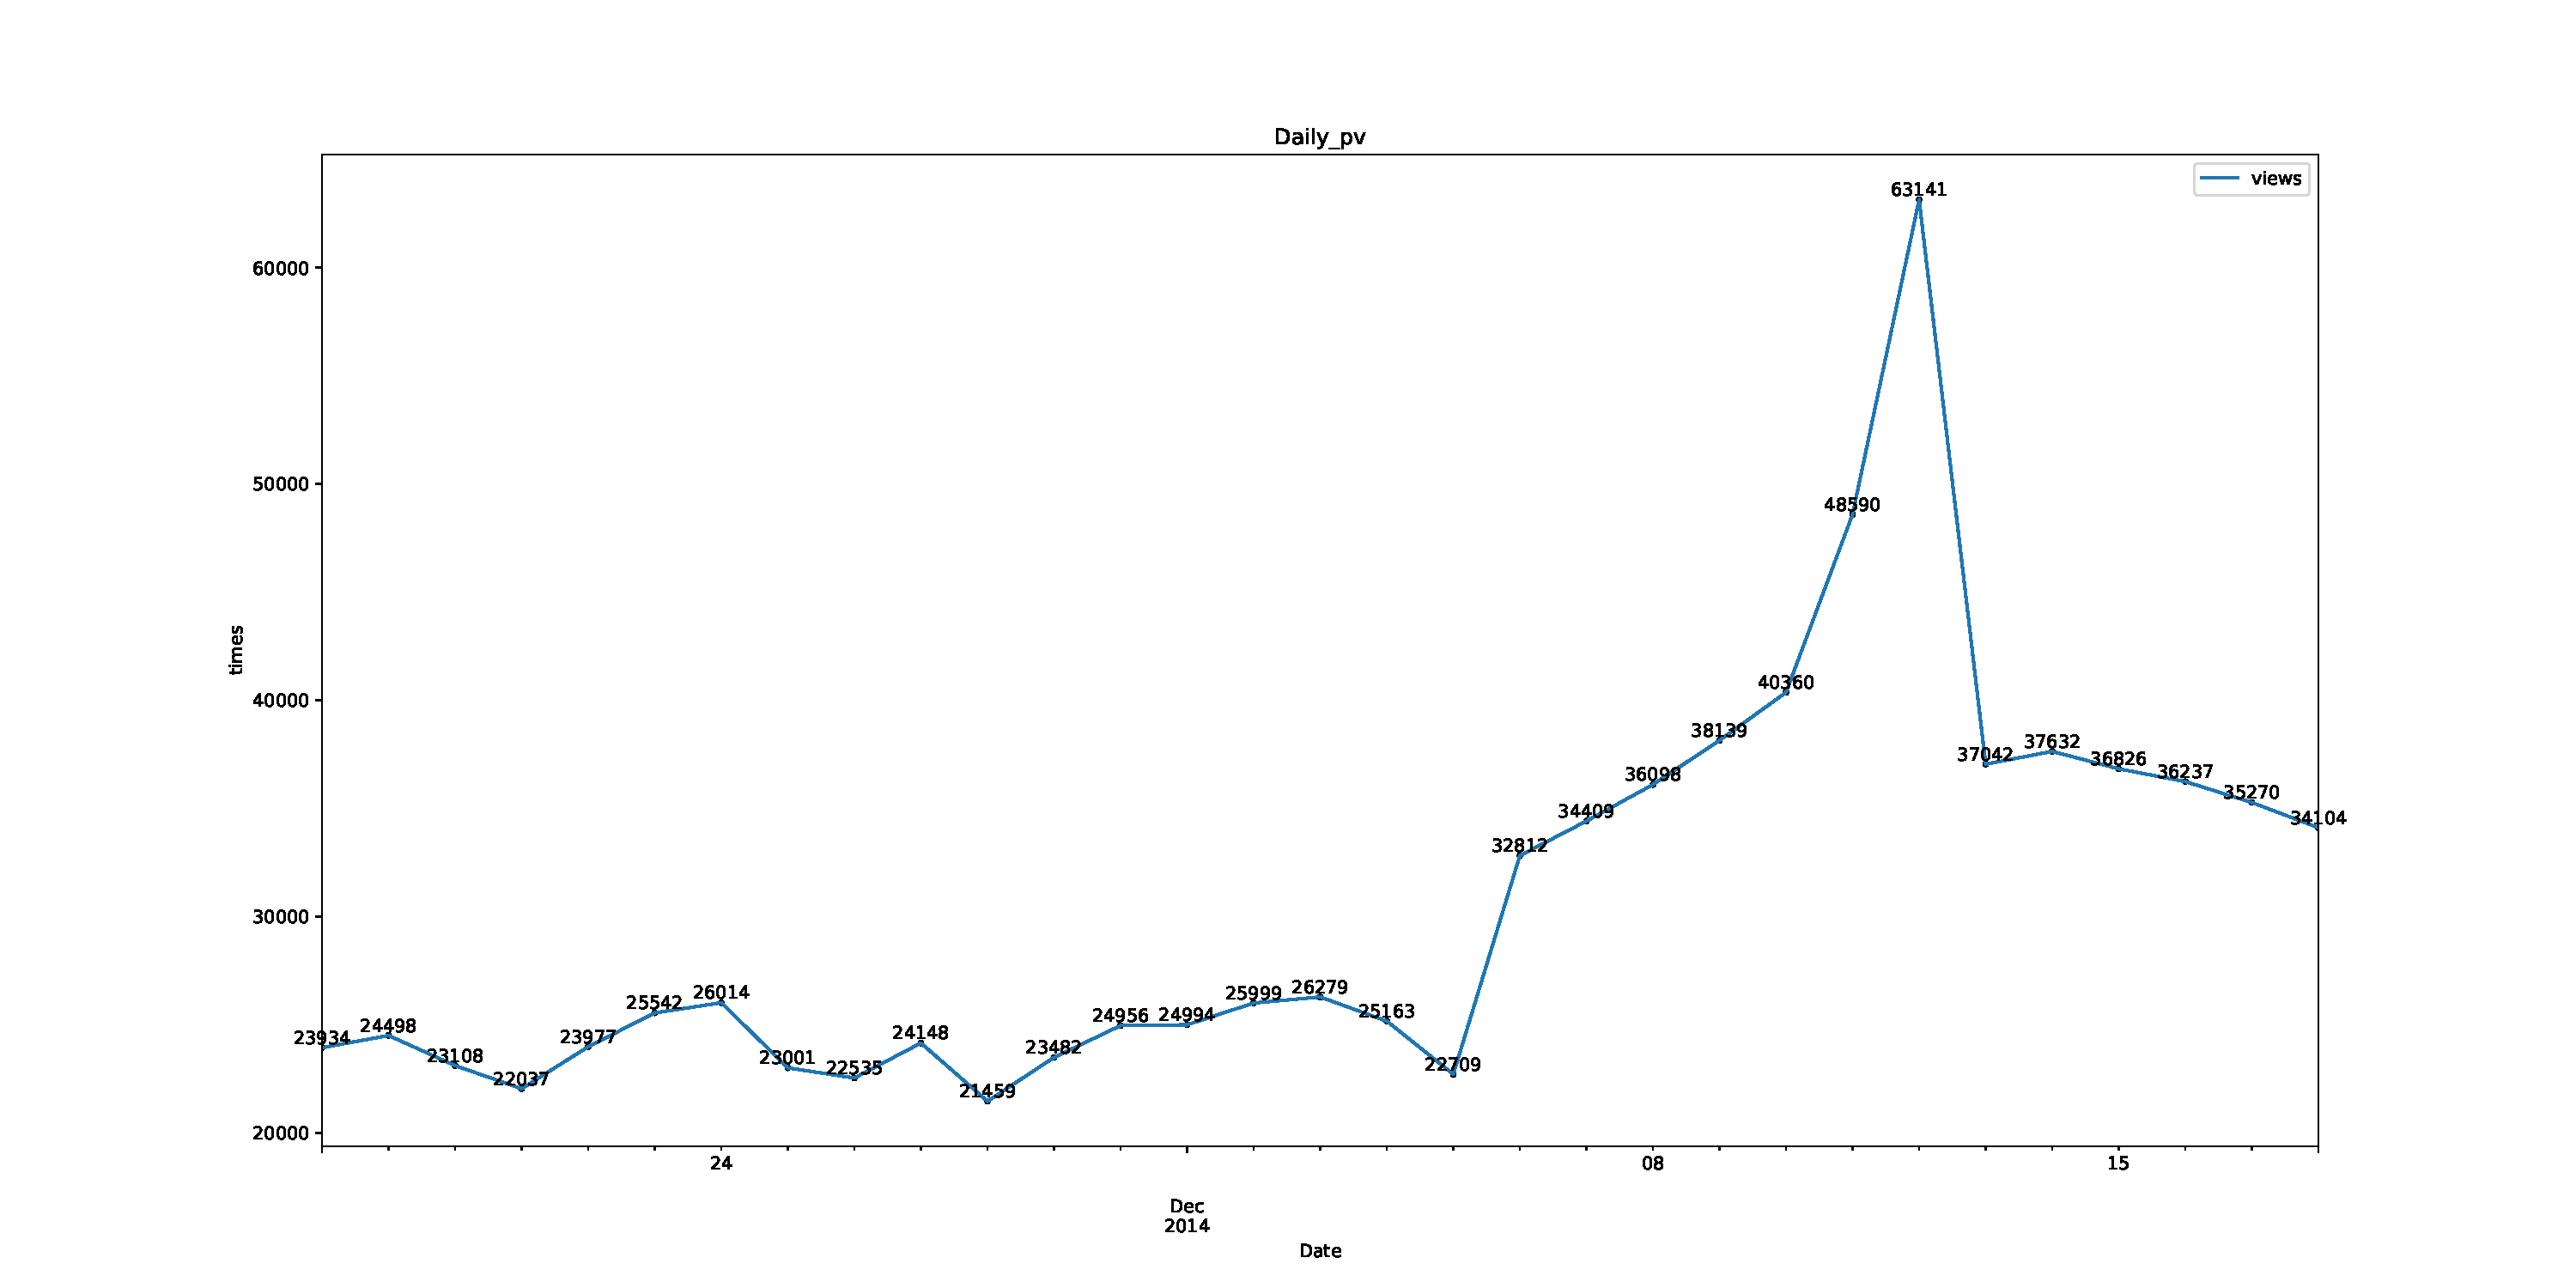
\includegraphics[width=1\textwidth]{./daily_pv.pdf}
	\caption{日浏览人次}
	\label{Fig.Daily_view}
\end{figure}

\begin{figure}[H]
	\centering
	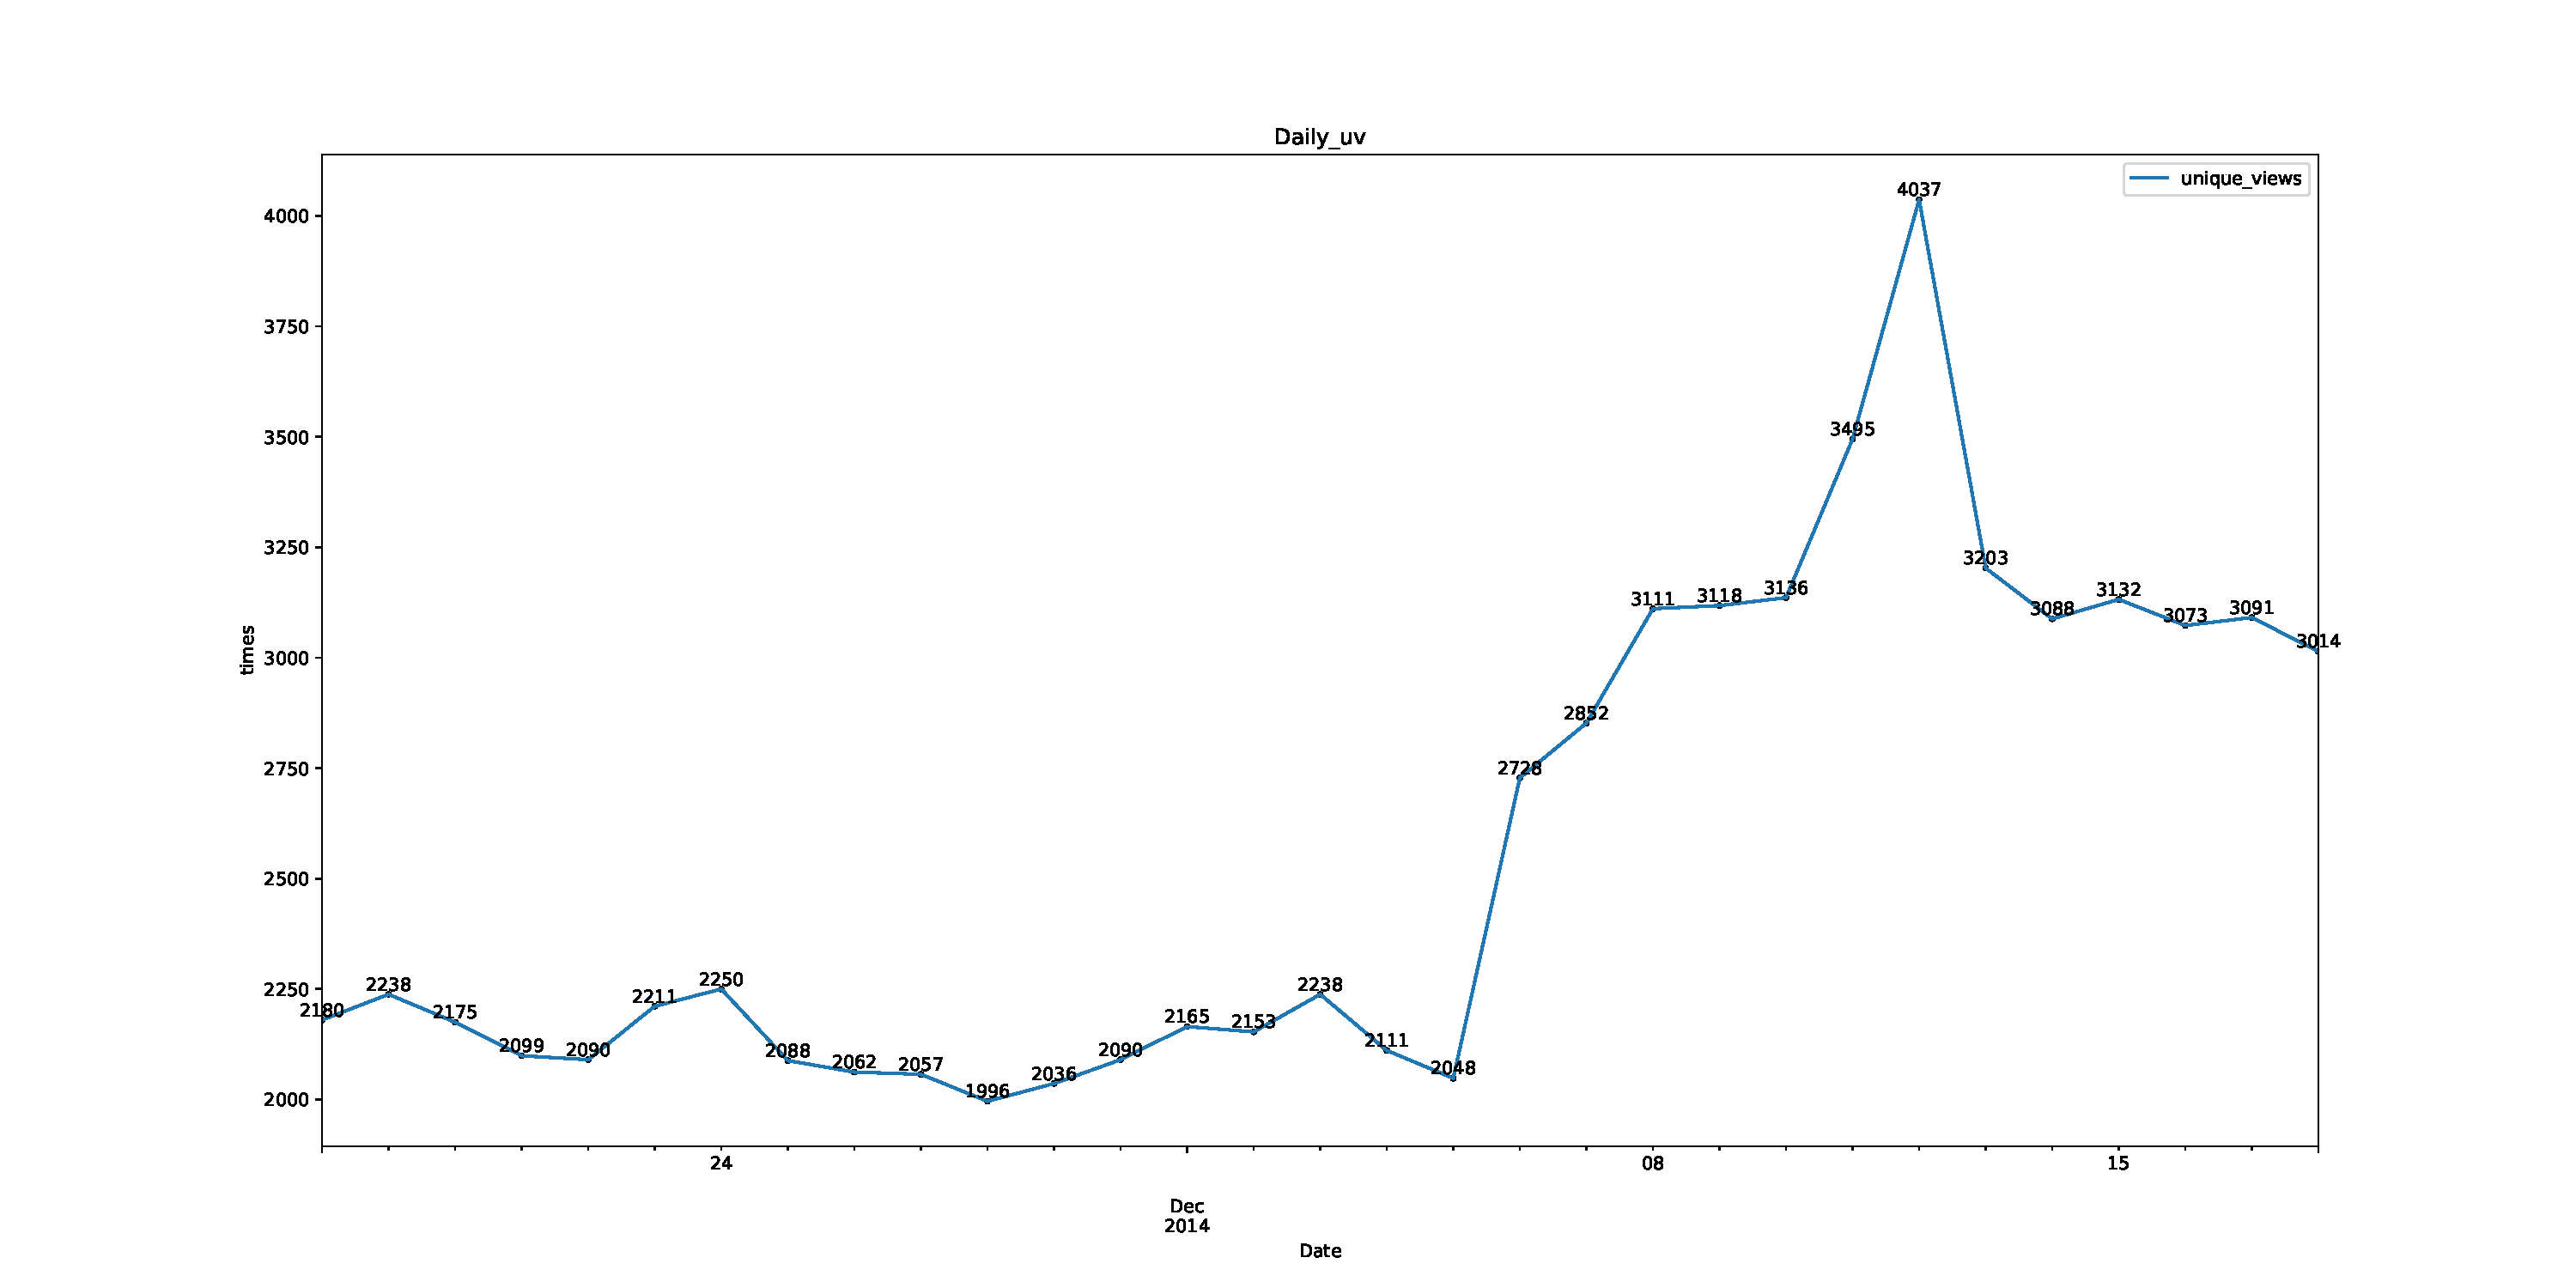
\includegraphics[width=1\textwidth]{./daily_uv.pdf}
	\caption{日浏览去重人数}
	\label{Fig.Daily_unique_view}
\end{figure}

\begin{figure}[H]
	\centering
	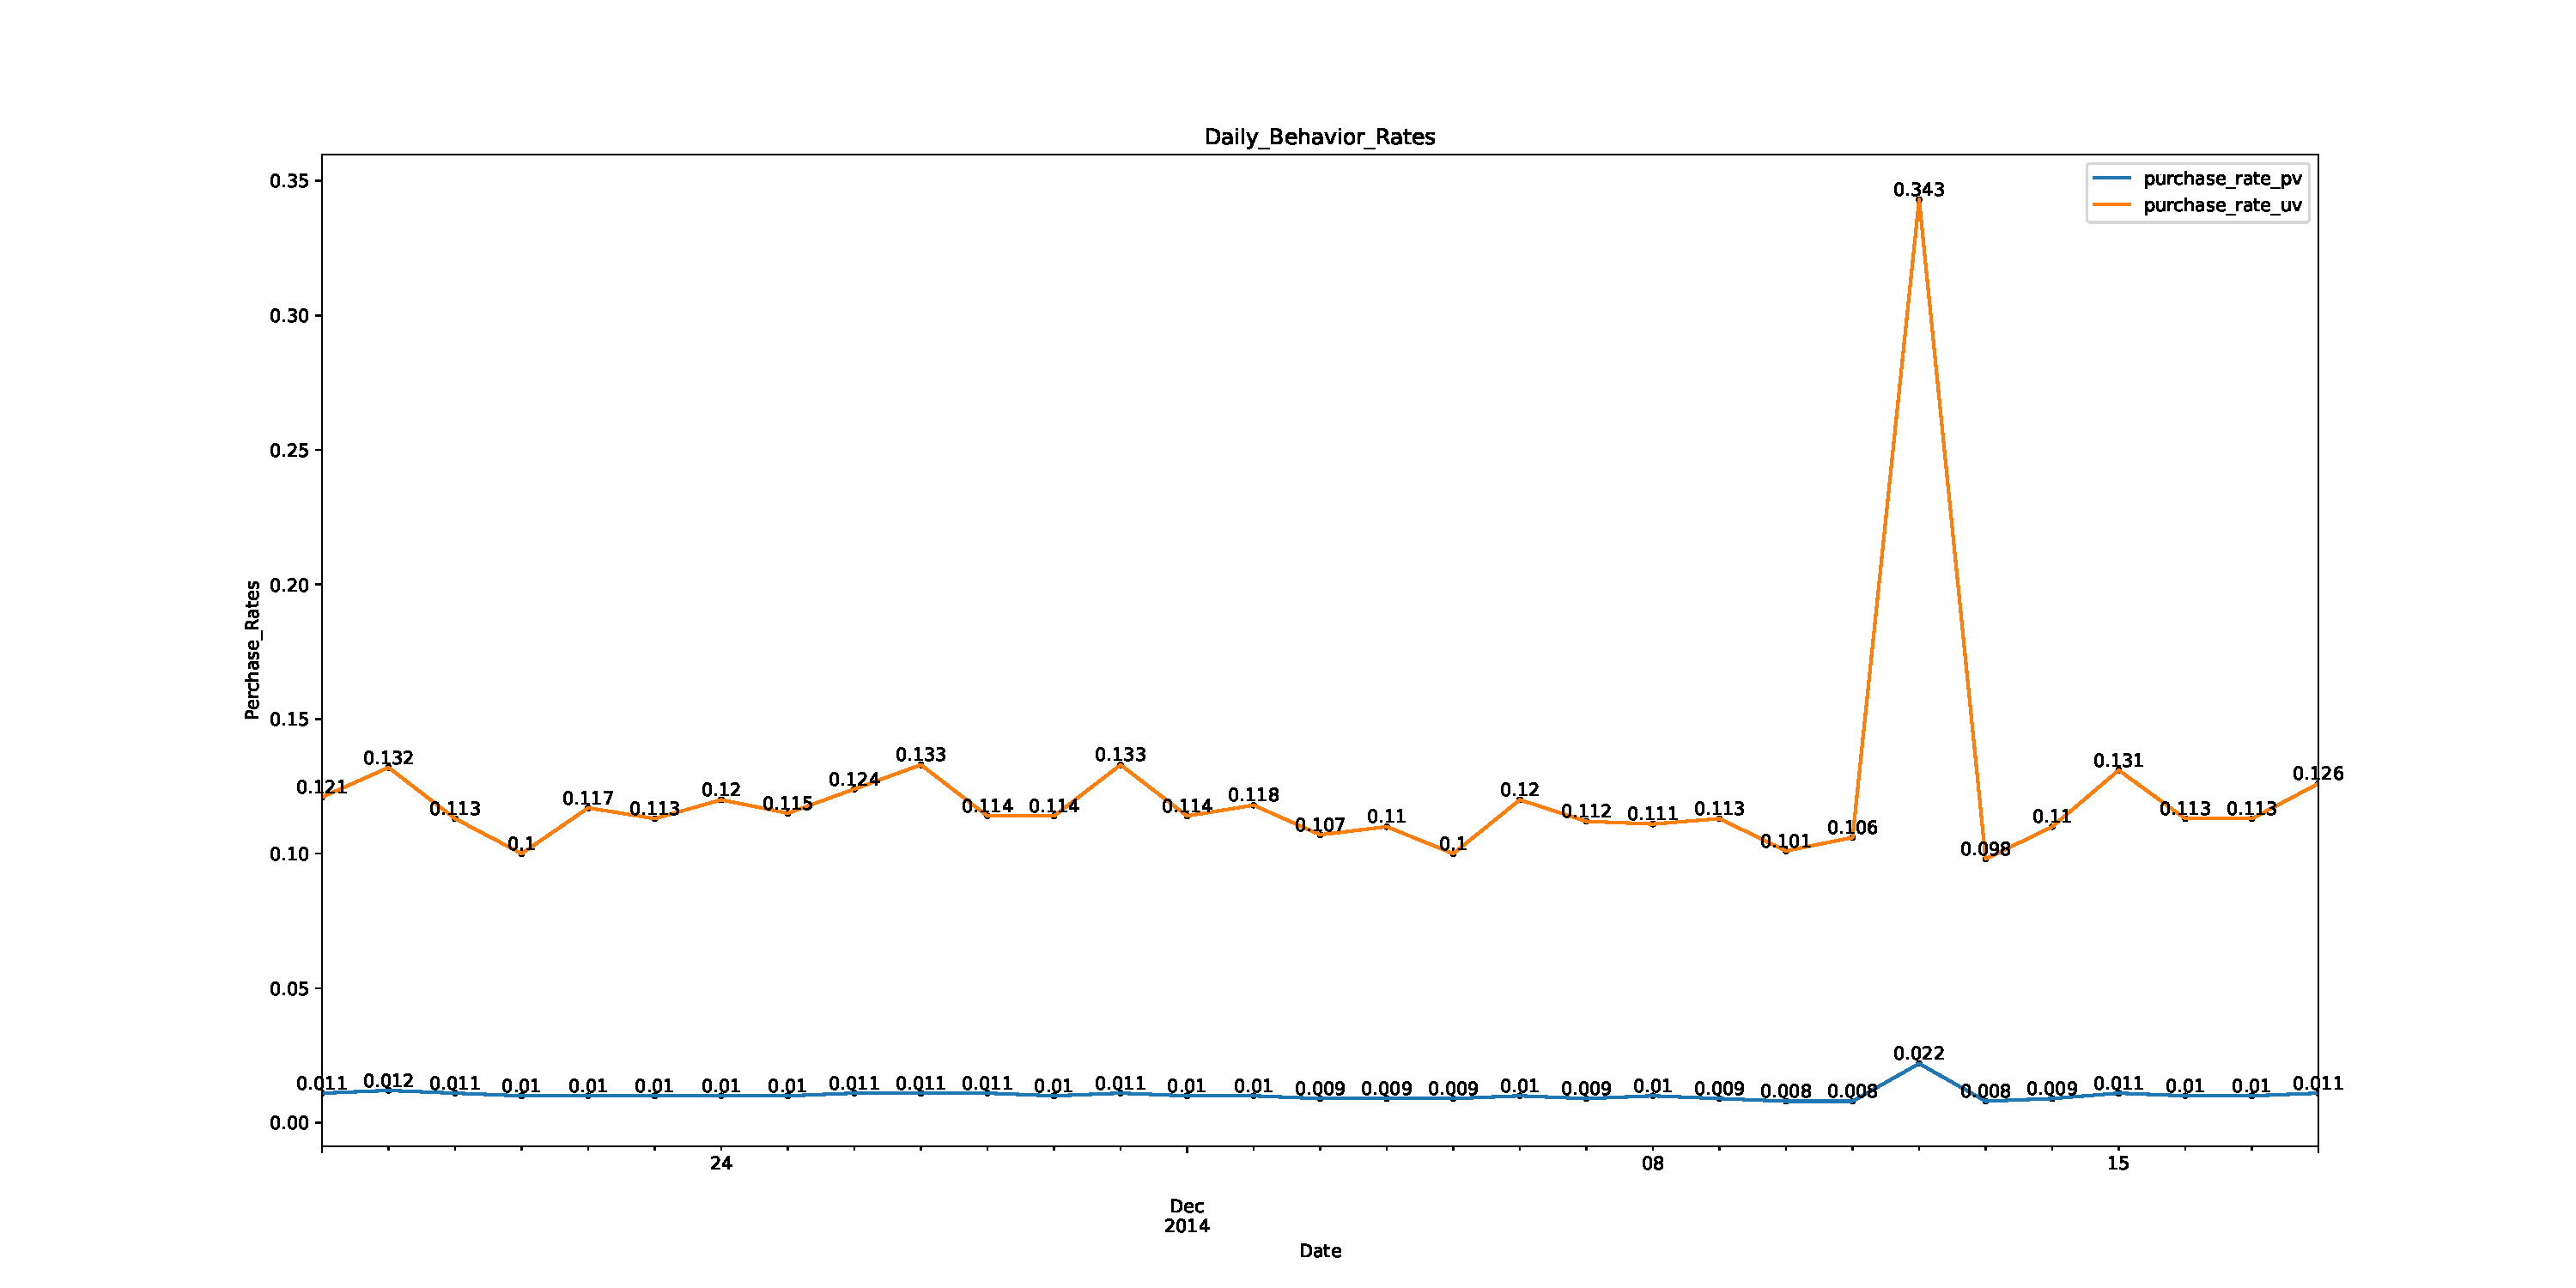
\includegraphics[width=1\textwidth]{./purchase_rate.pdf}
	\caption{付费率(pv和uv)(付费人数/浏览人数)}
	\label{Fig.purchase_rate}
\end{figure}

\begin{figure}[H]
	\centering
	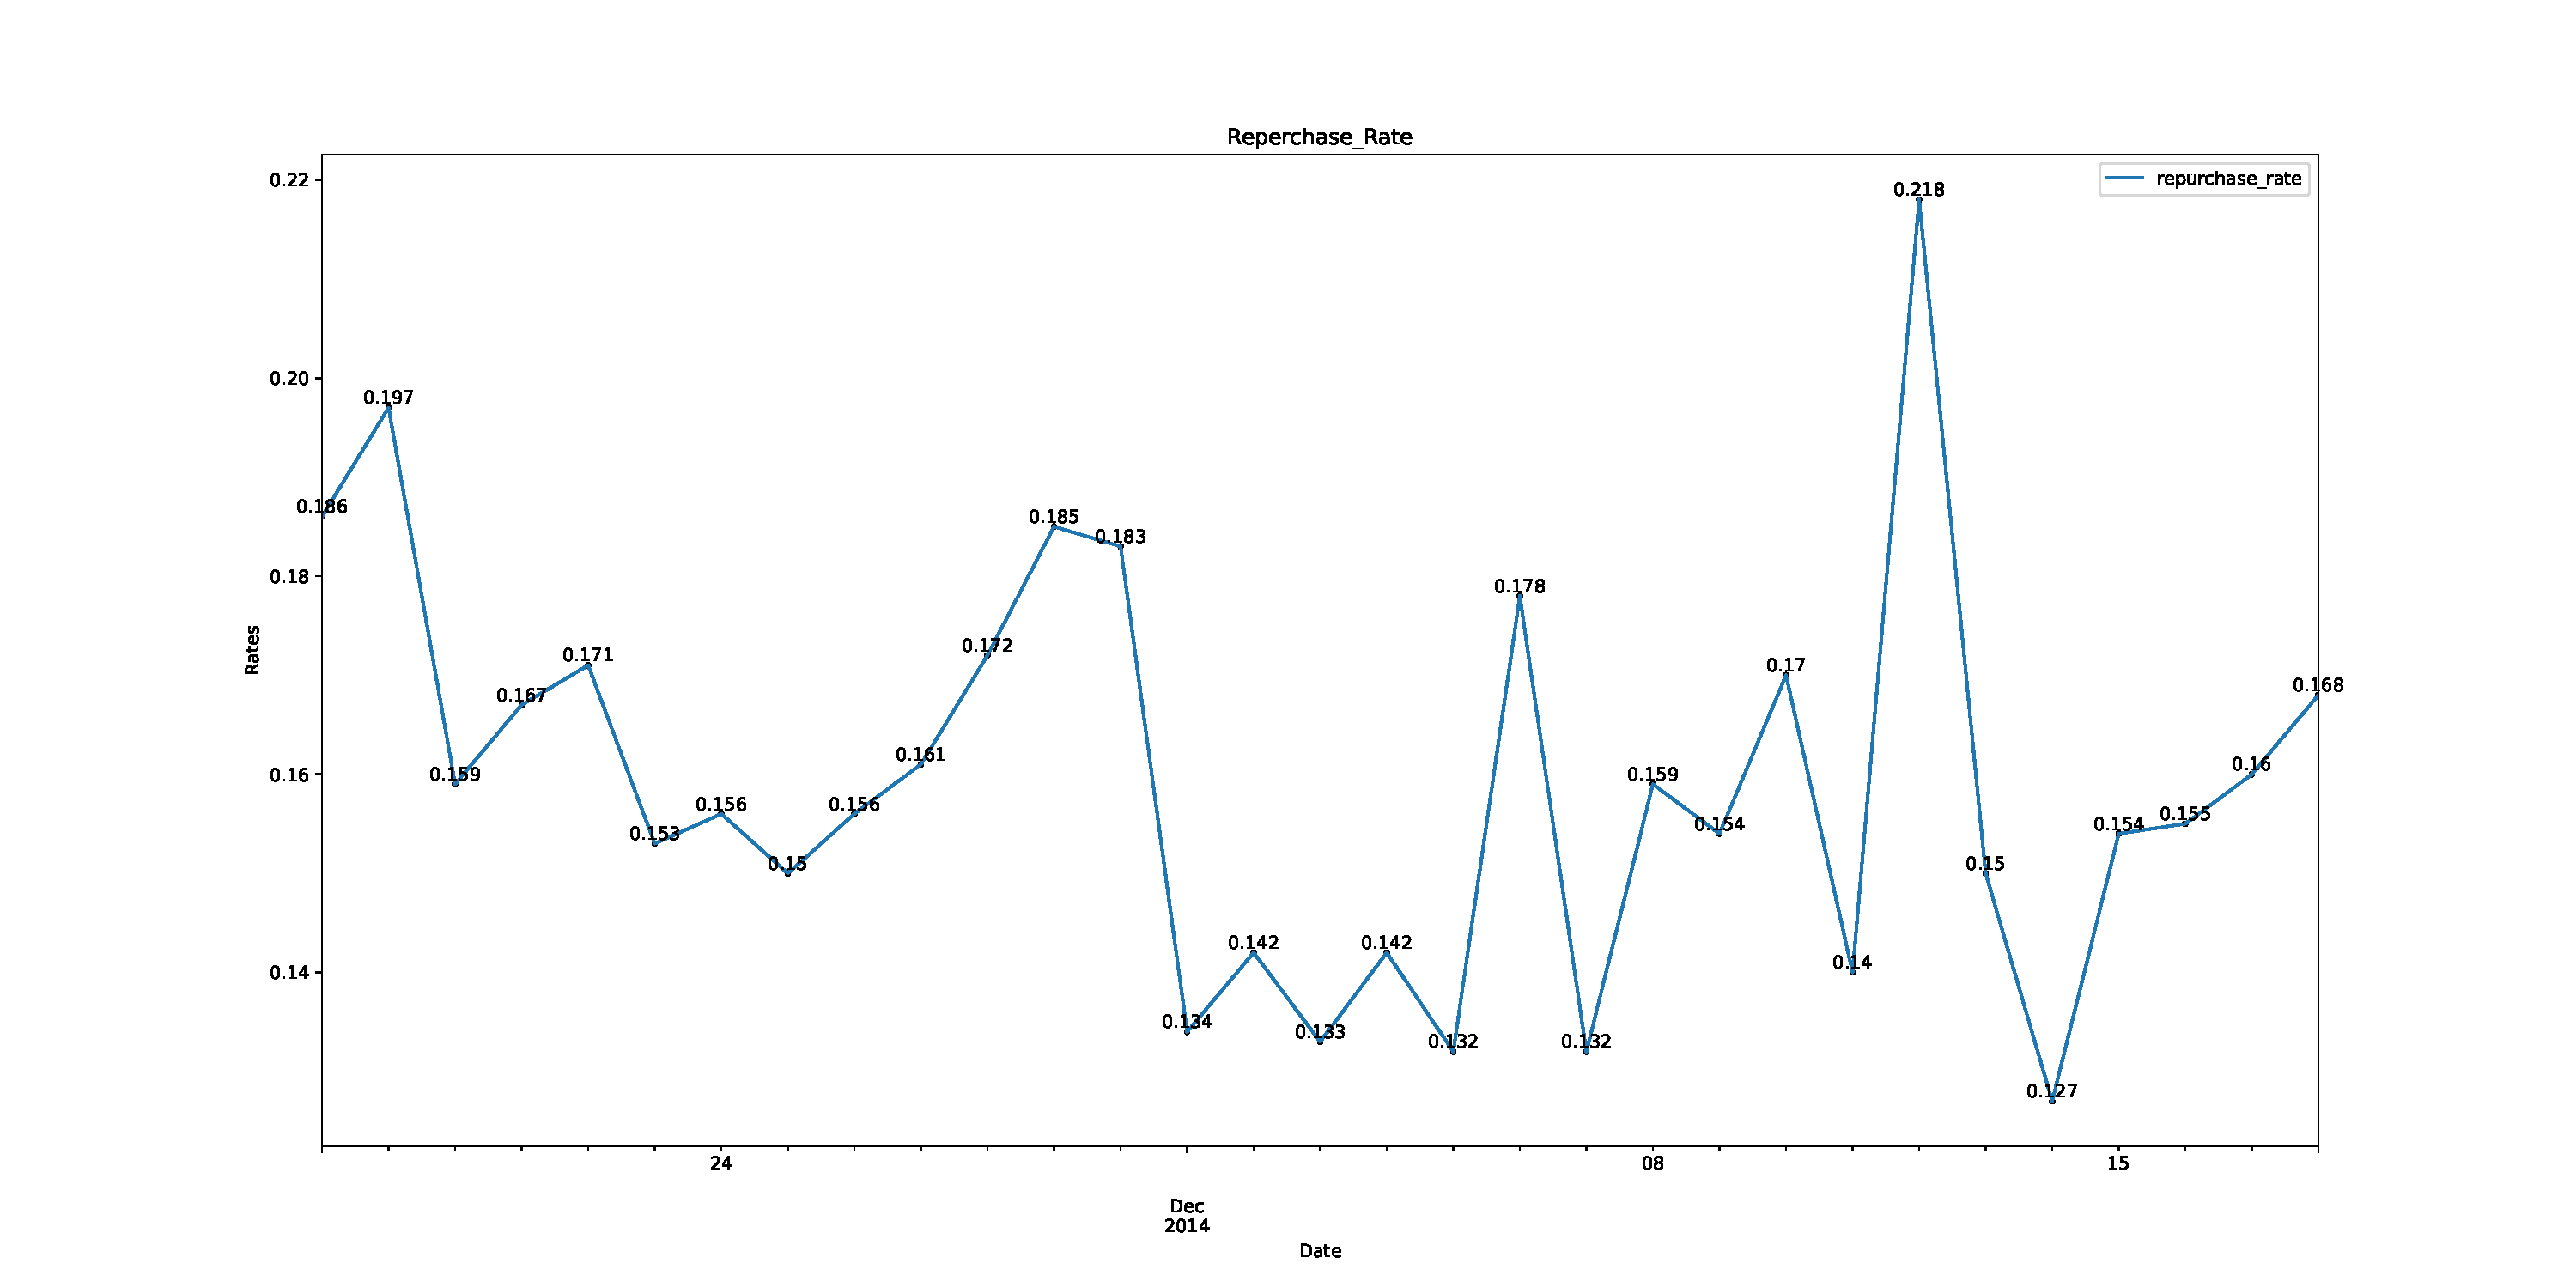
\includegraphics[width=1\textwidth]{./reperchase_rate.pdf}
	\caption{复购率(购买2次以上人数/购买人数)}
	\label{Fig.repurchase_rate}
\end{figure}

\begin{figure}[H]
	\centering
	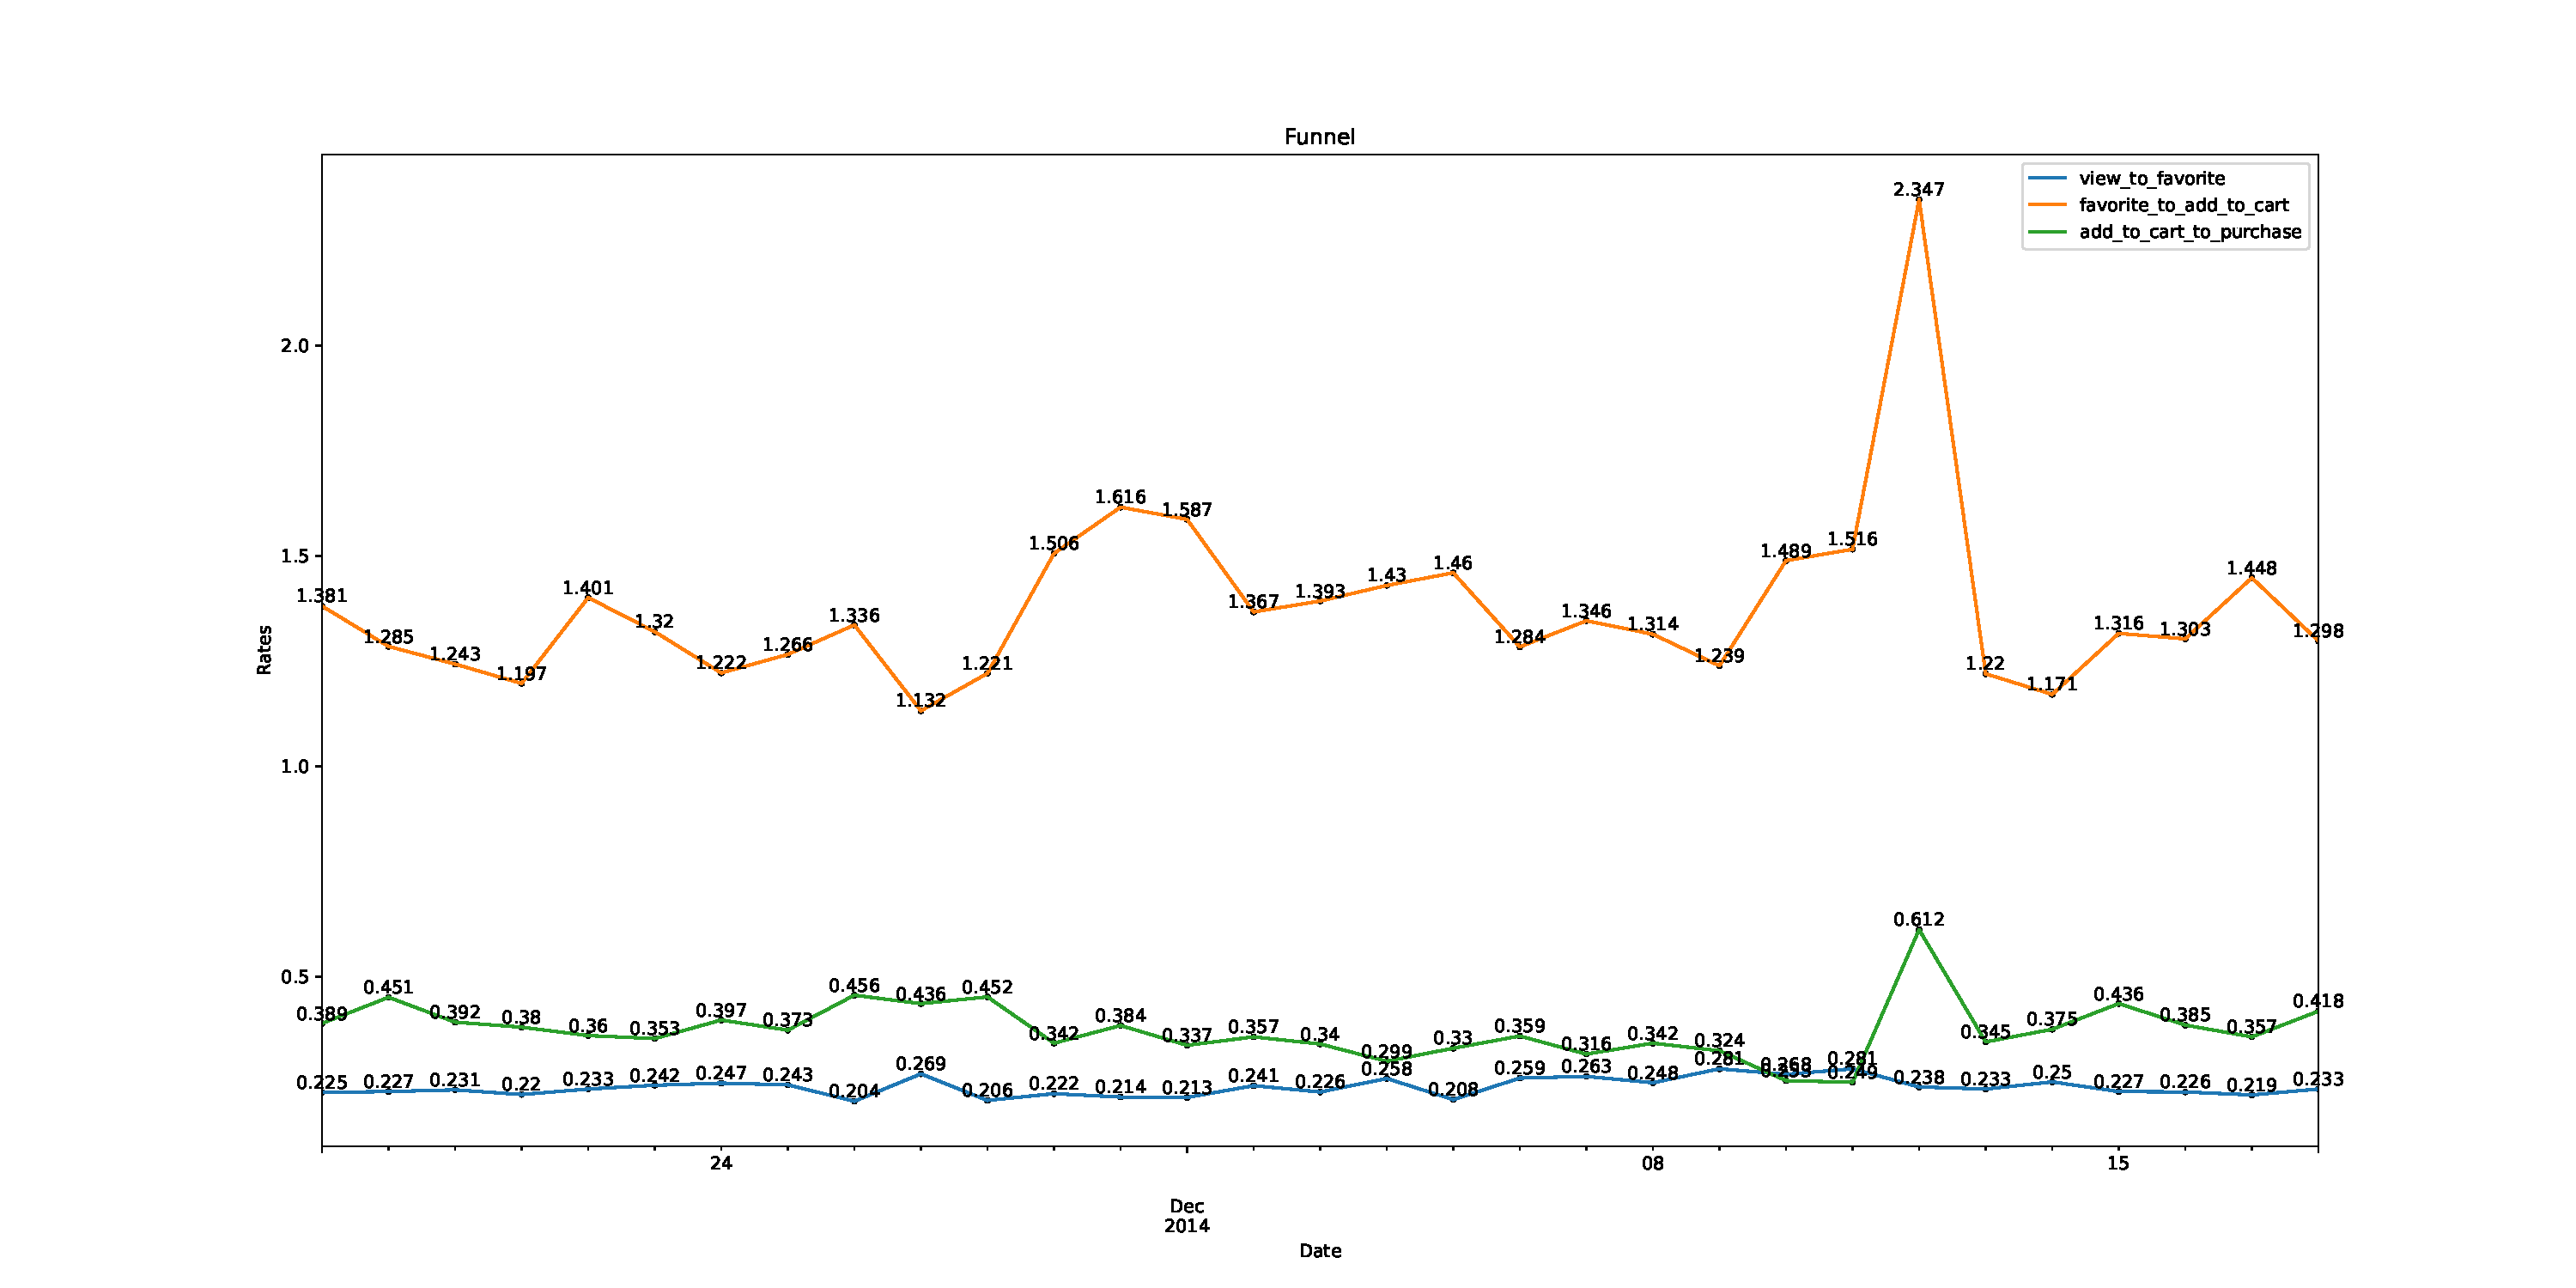
\includegraphics[width=1\textwidth]{./funnel.pdf}
	\caption{漏斗流失(浏览->收藏、收藏->加购物车、加购物车->购买)}
	\label{Fig.funnel}
\end{figure}

\newpage

\noindent2. 在哪一天发生了购买量的突增和突降,可能的原因是什么(指标拆解和维度拆解)

{\bf指标拆解}: 每日购买量 = 日浏览去重人数(uv) * 每日购买率(purchase\_rate(uv))

\begin{figure}[H]
	\centering
	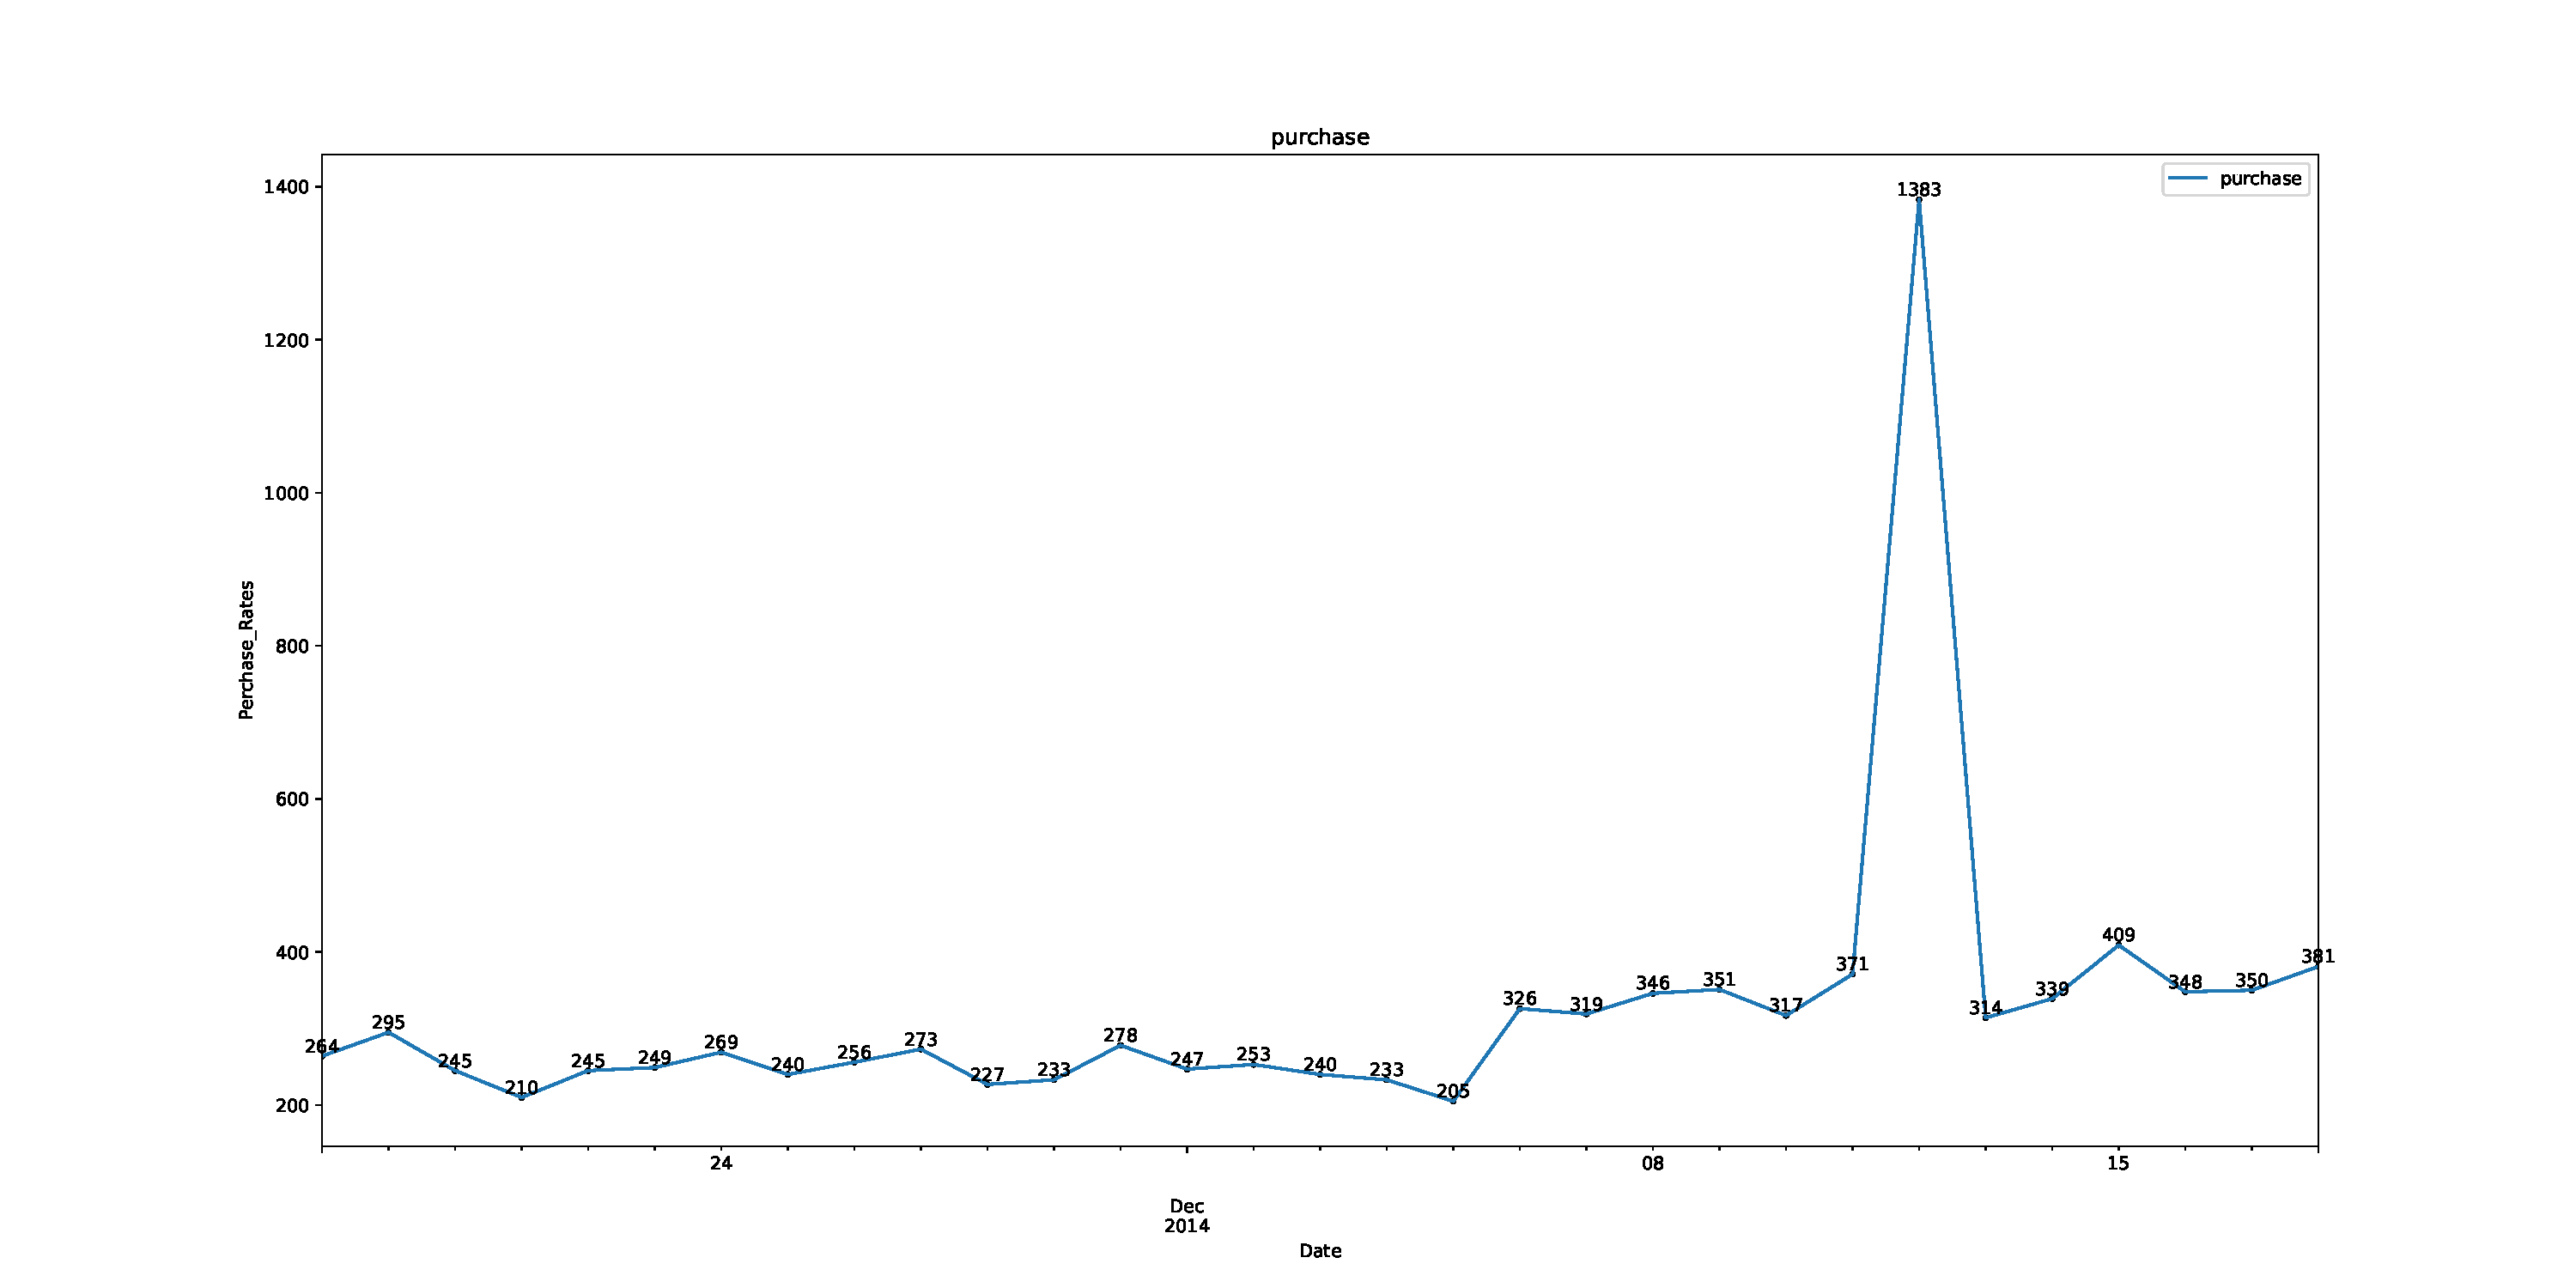
\includegraphics[width=1\textwidth]{./purchase.pdf}
	\caption{每日购买量}
\end{figure}

\begin{figure}[H]
	\centering
	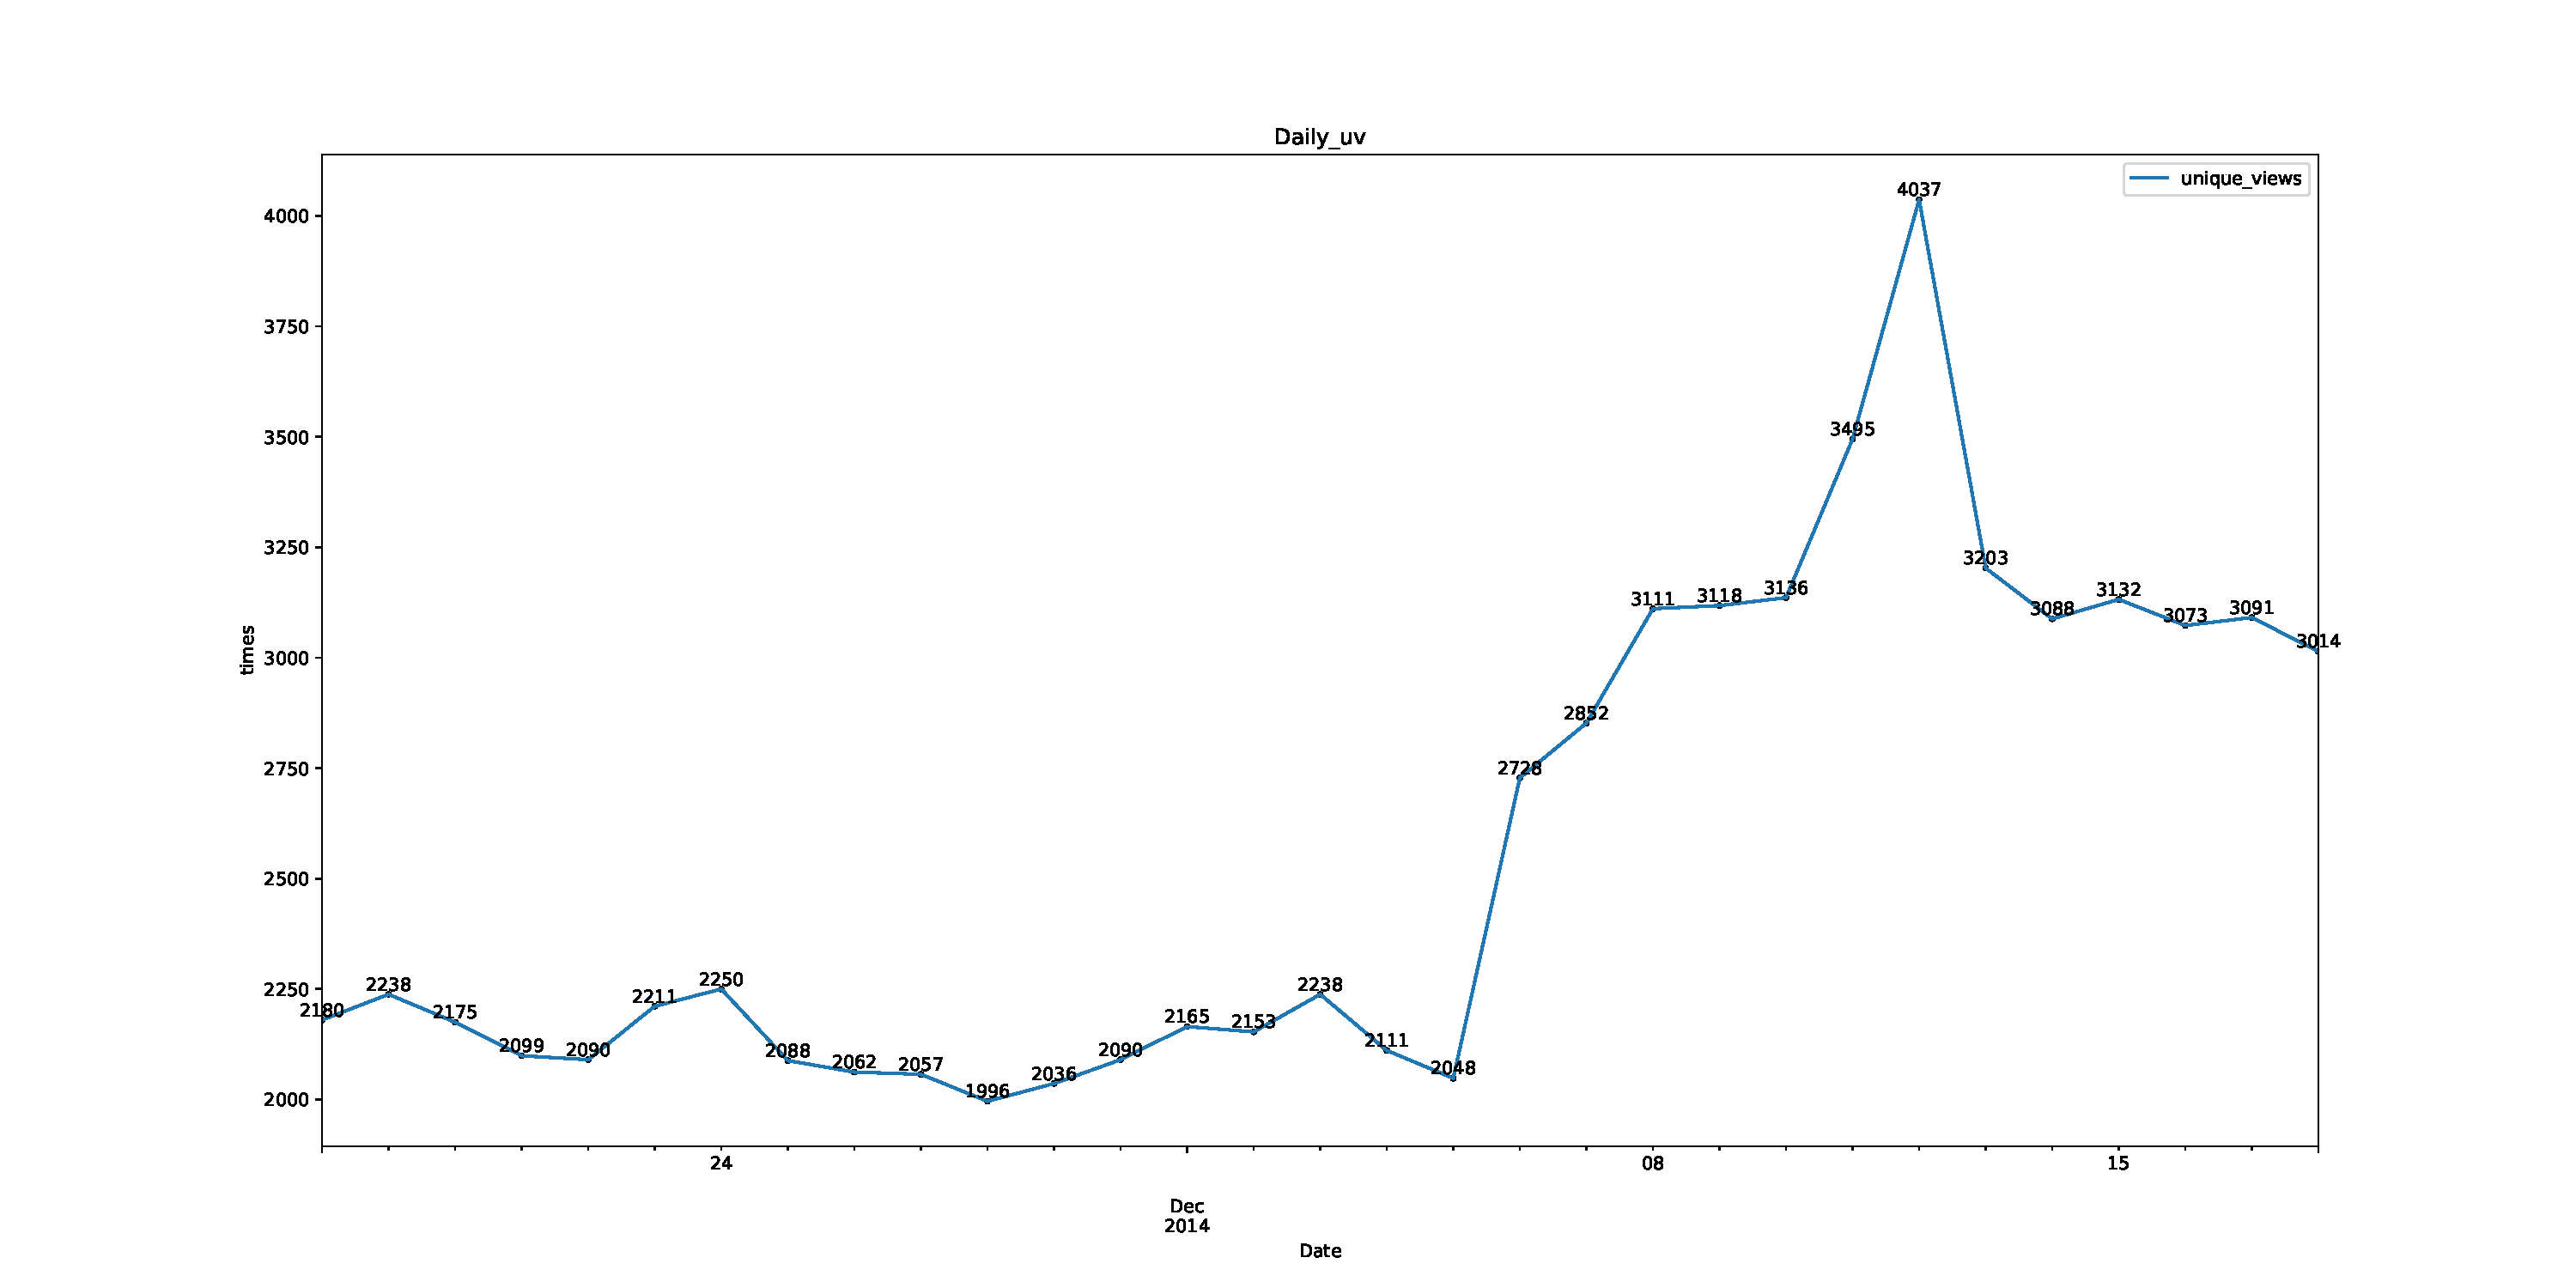
\includegraphics[width=1\textwidth]{./daily_uv.pdf}
	\caption{日浏览去重人数}
\end{figure}

\begin{figure}[H]
	\centering
	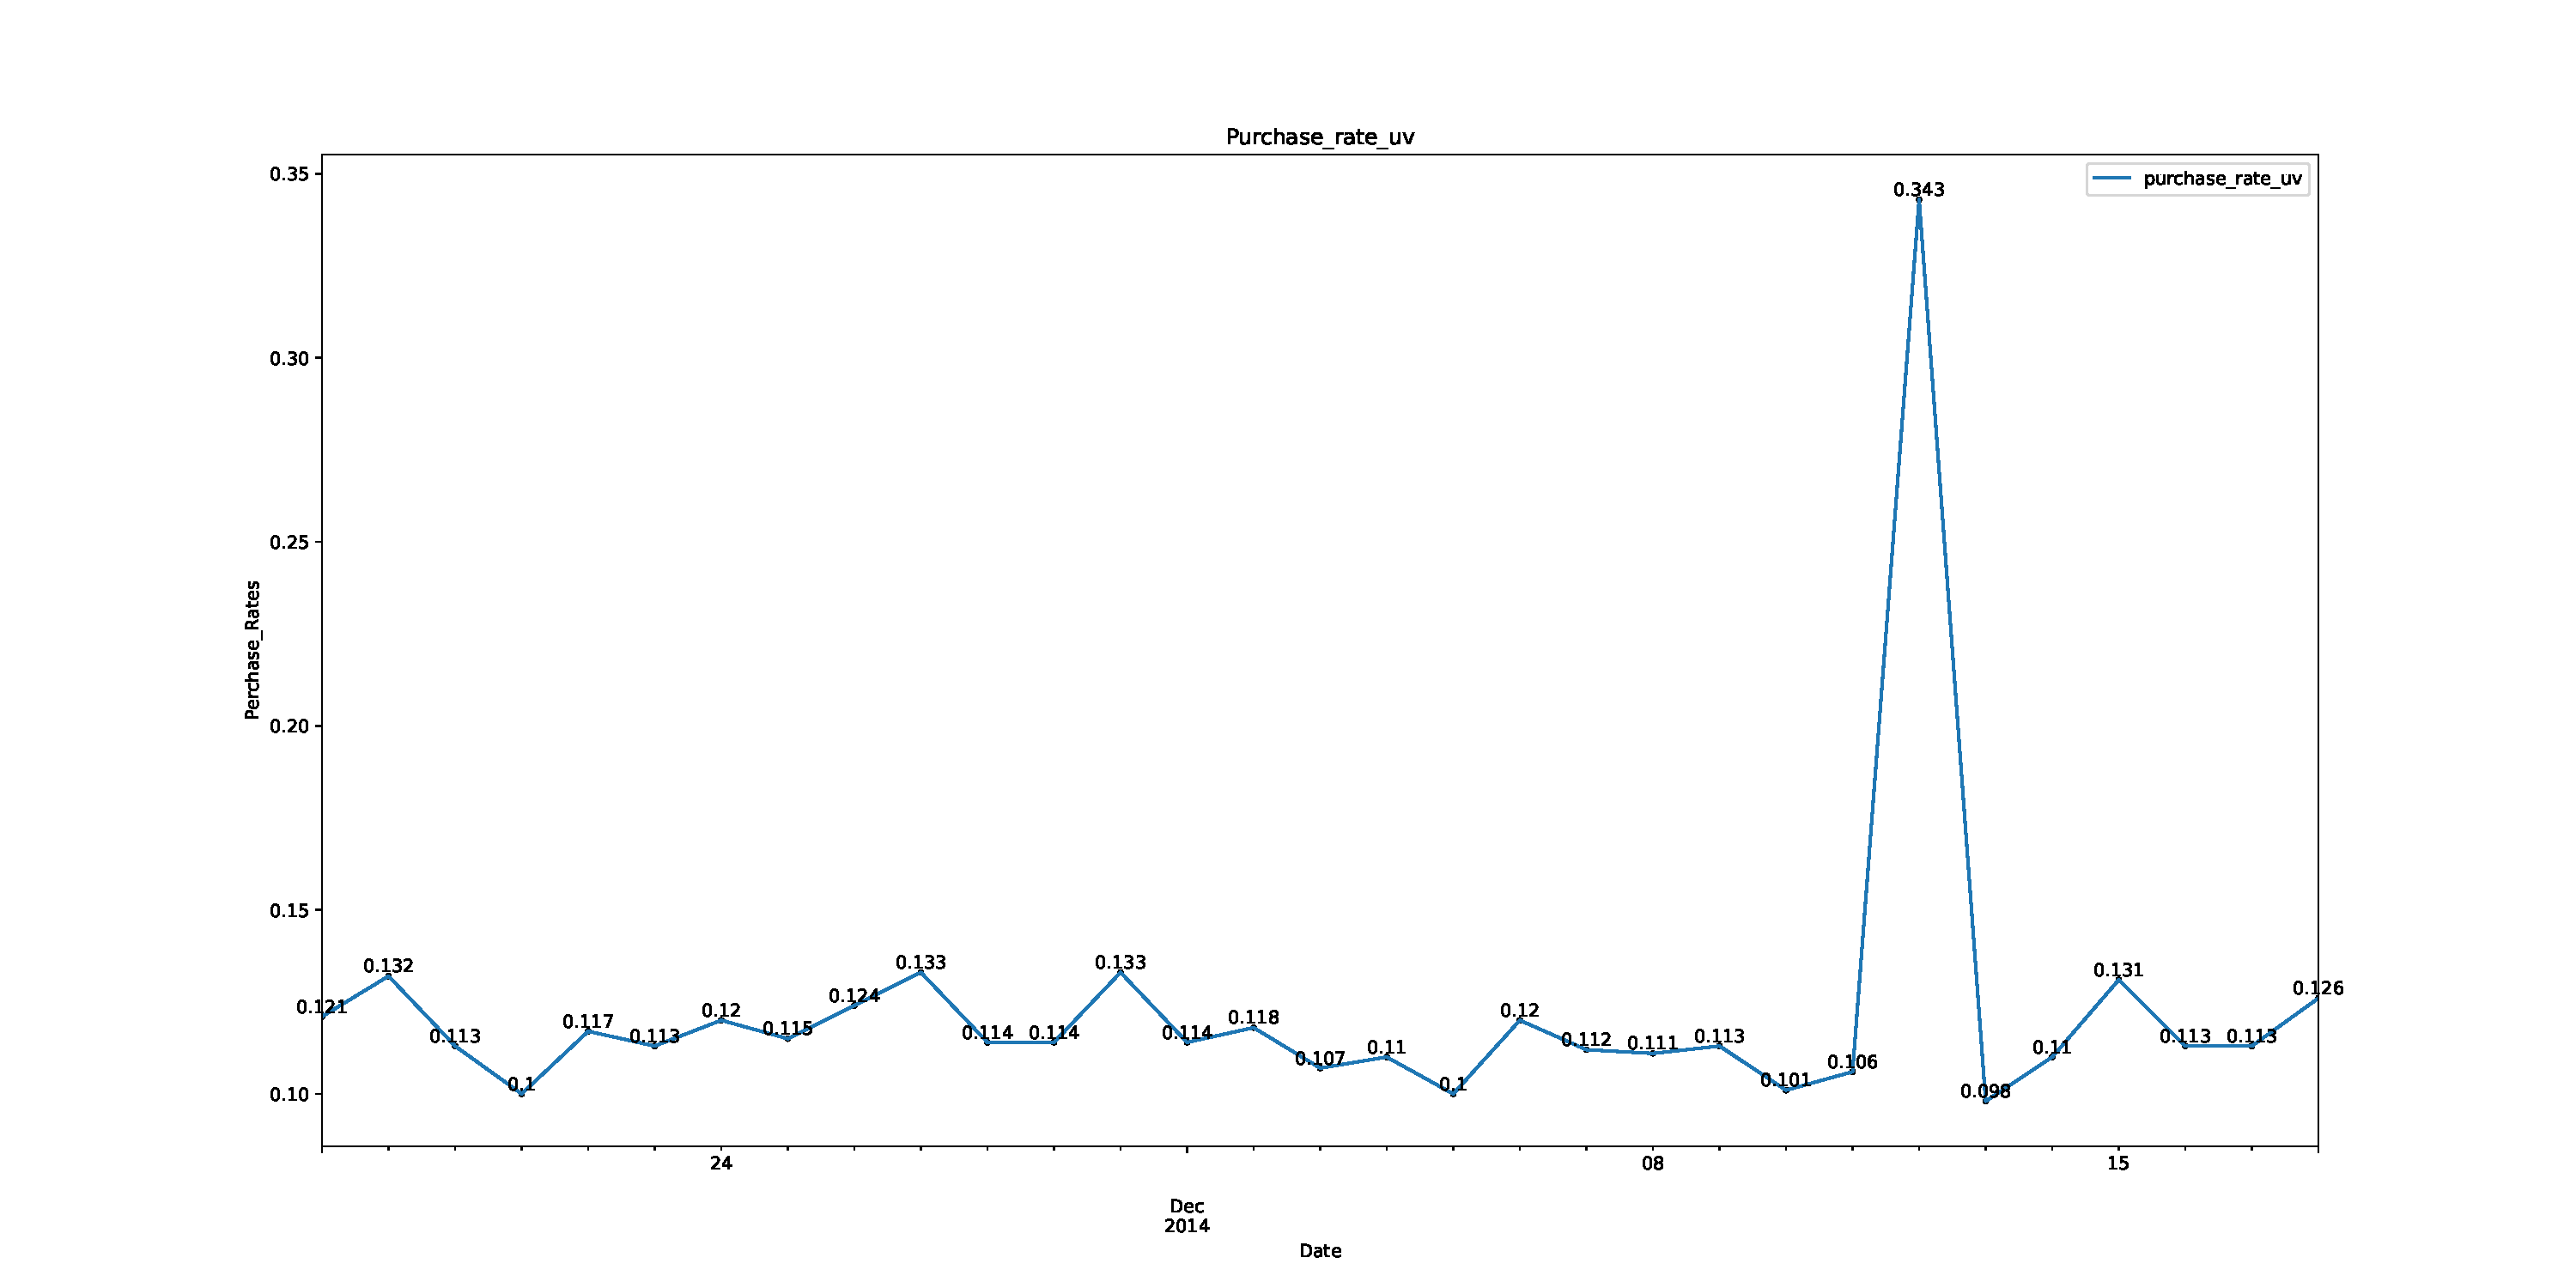
\includegraphics[width=1\textwidth]{./purchase_rate_uv.pdf}
	\caption{每日购买率(purchase\_rate(uv))}
\end{figure}

能通过三张图发现, 在12月12号, 日浏览去重人数和每日购买率都有一个很明显的增长\\

{\bf维度拆解}: 购买用户 : 会员, 用户性别

\begin{figure}[H]
	\centering
	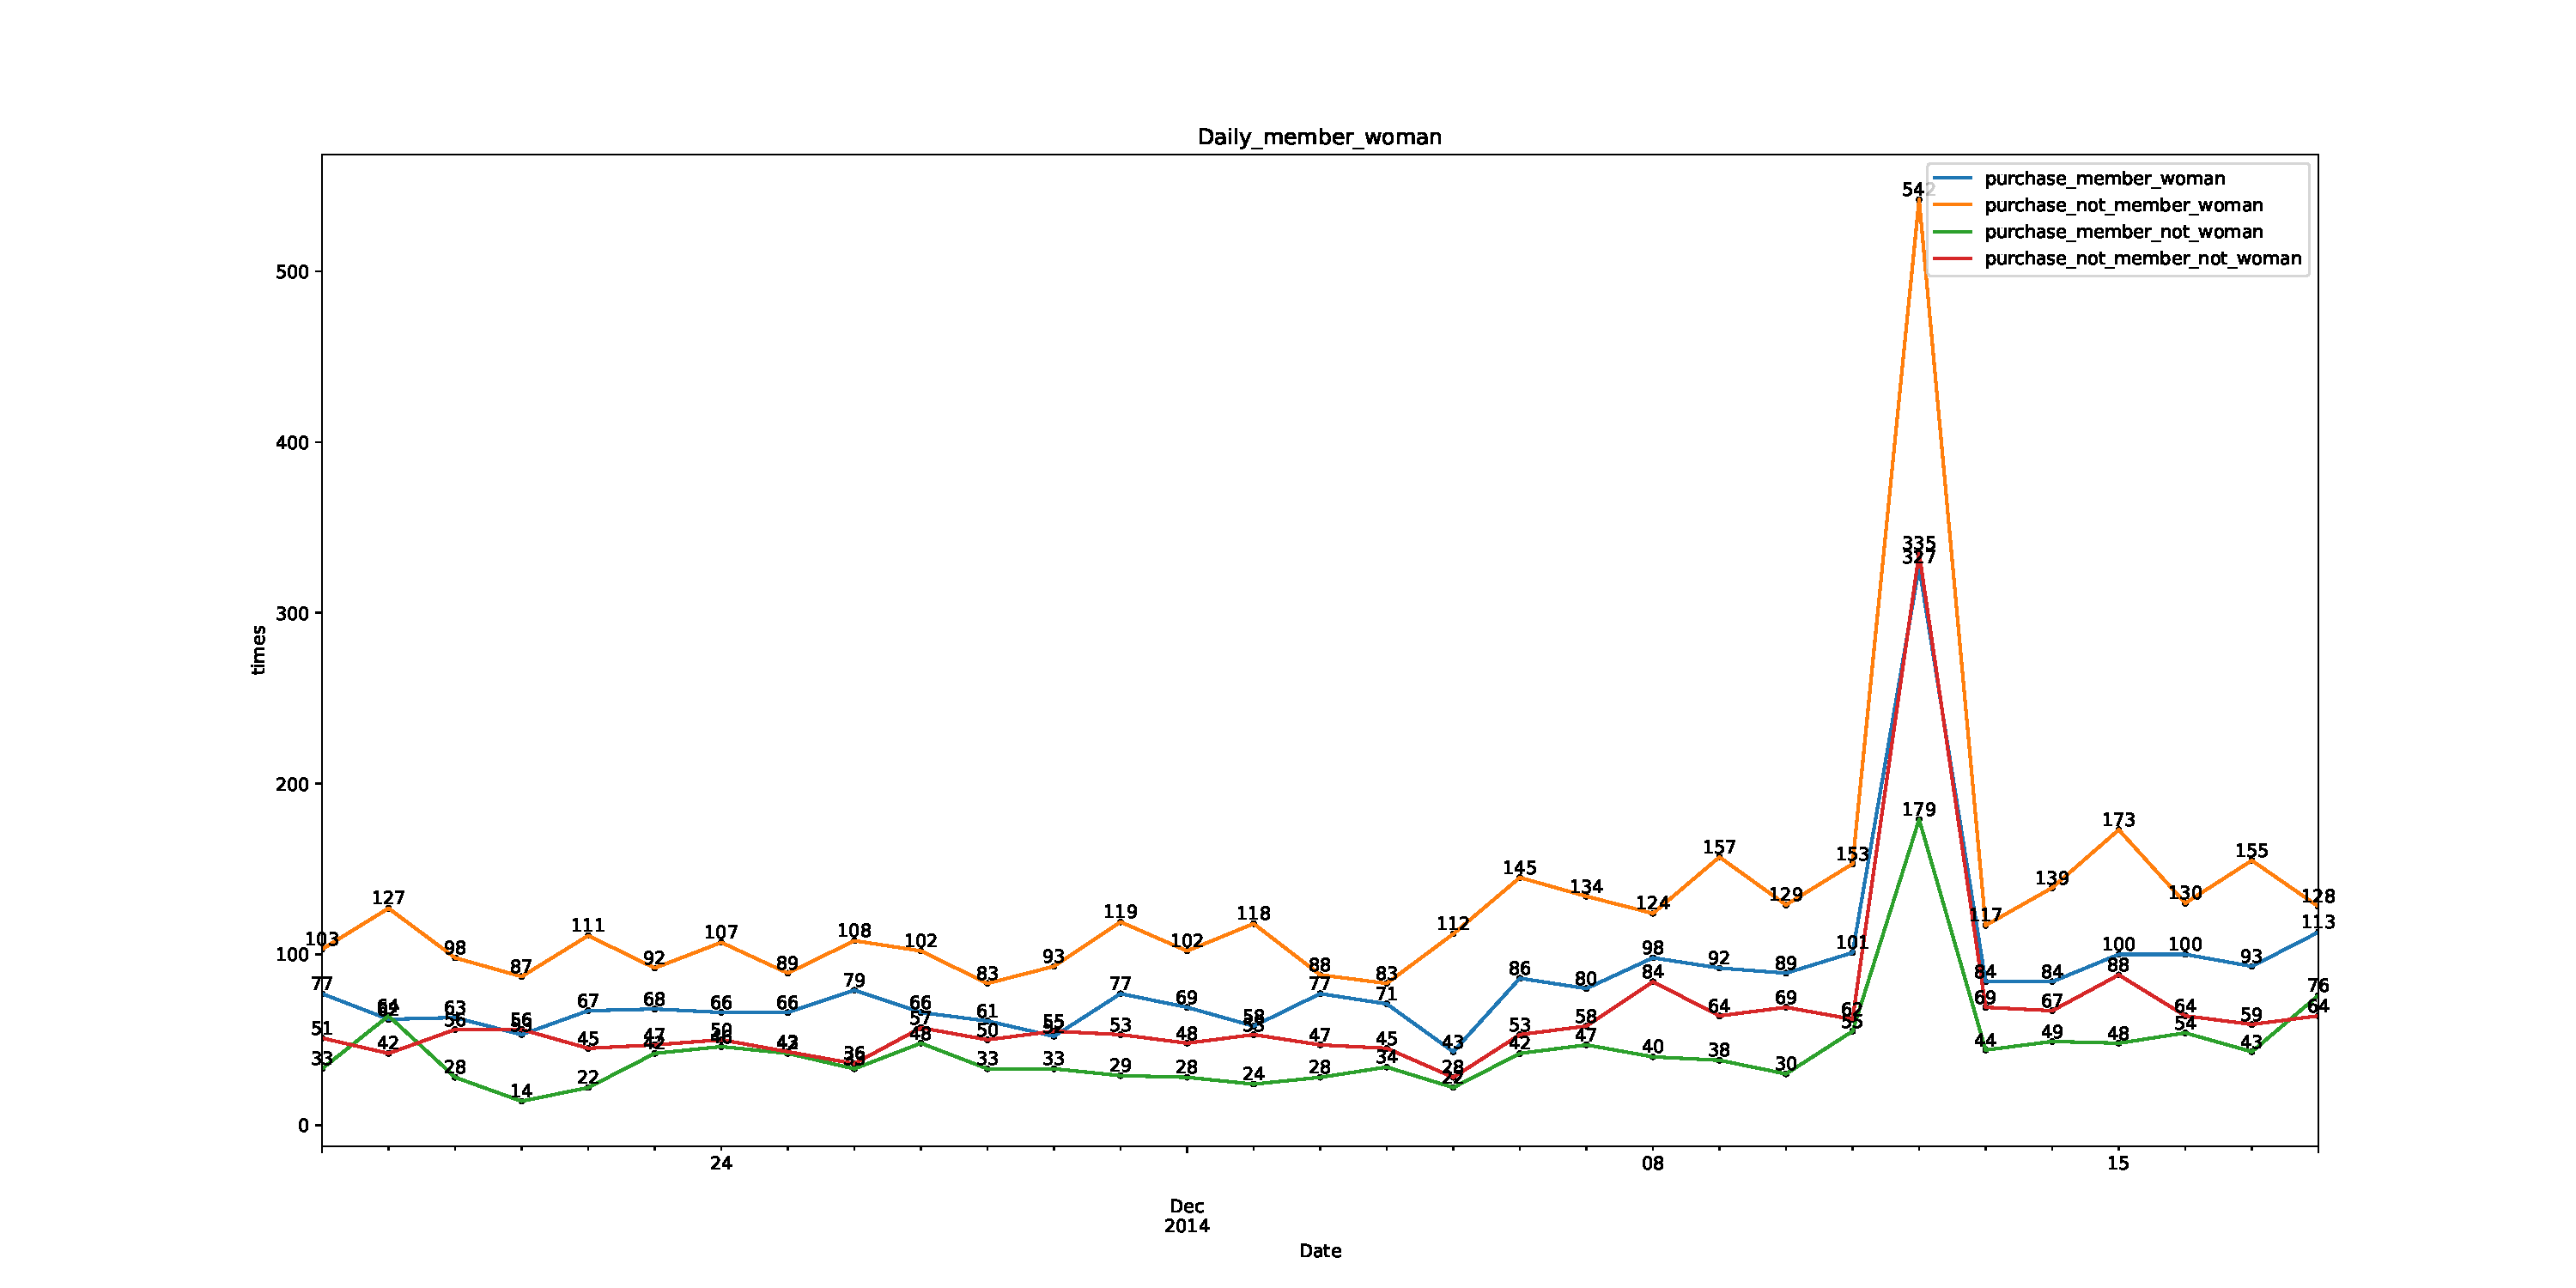
\includegraphics[width=1\textwidth]{./daily_member_woman.pdf}
	\caption{会员和性别带来的购买差异}
\end{figure}

能通过对比发现, 在12月12号, 无论是否是会员或者为女性, 购买率都有一个大幅度的增长

其中, 总趋势是 非会员女性 > 会员女性 > 非会员男性 > 会员男性\\

{\bf可能原因分析}: 

1. \href{https://baike.baidu.com/item/%E5%8F%8C%E5%8D%81%E4%BA%8C%E8%B4%AD%E7%89%A9%E7%8B%82%E6%AC%A2%E8%8A%82/23196918}{\underline{双12节日促销}}, 商品打折(尤其是针对女性商品)带来了更多的浏览量与购买量

2. 12月12日左右, 某件商品热度增加, 带来了更多的浏览量与购买量

\end{document}